\chapter{\TeX{} 简介}{Introduction of \TeX}
\label{cha:IntroductionOfTeX}

\TeX{} \index{\TeX} 是一个格式化排版系统, 它一问世便以其排版效果的高质量震动整个
出版界. 尤其是在排版含有大量数学公式的科技文献方面更显示了它的优越性. \TeX{}
\index{\TeX} 还是一个程序源代码公开的免费排版系统, 因此吸引了许多计算机专家及
\TeX{} \index{\TeX} 爱好者为之添砖加瓦.

20 世纪 60 年代, 著名计算机专家和数学家, 斯坦福大学 Donald E. Knuth \index{Knuth}
(读音: ka-nooth) 教授准备出系列专著《The art of computer programming》, 前三卷已
经出版. 当他正在撰写第四卷时, 出版社拿来了第二卷的第二版书样给他过目, 结果令他大
失所望, 因为当时出版社的印刷技术没有使他的书稿更好看, 反而变糟了, 尤其是在数学公
式和字体上面的缺陷更令他无法接受. 于是他就打算自己写一个既能供科学家编排手稿又符
合出版社印刷要求的高质量的计算机排版系统 \index{计算机排版系统}.

\begin{figure}
  \centering
  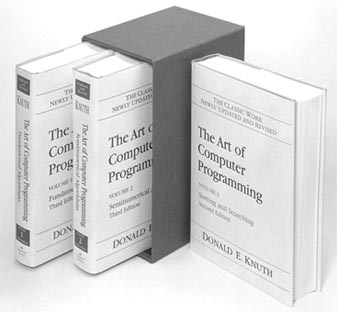
\includegraphics[width=6cm]{TheArtOfComputerProgramming.jpg}\\
  \caption{计算机编程的艺术}{The art of computer programming}
  \label{fig:TheArtOfComputerProgramming}
\end{figure}

Knuth \index{Knuth} 教授于 1977 年开始构造 \TeX{} \index{\TeX} 系统, 并为该系统
设计了一个字符字体生成软件: METAFONT\index{METAFONT}, 在标准的 \TeX{} \index{\TeX}
系统中包含有 75 种不同尺寸的字体, 且每种字体有 8 种不同的缩放比例.

1982 年 \TeX{} \index{\TeX} 系统成功开发出版, 之后又有几次升级. Knuth \index{Knuth}
教授用无理数 $\pi$ 的近似值作为 \TeX{} \index{\TeX} 系统的版本序号, $\mathrm{e}$
的近似值作为 METAFONT \index{METAFONT} 版本序号, 每升级一次其版号就增加一位数字,
不断地趋近于 $\pi$ 和 $\mathrm{e}$, 这也表达了 \TeX{} \index{\TeX} 不断追求完美
的愿望.

\TeX{} \index{\TeX} 的名称是由三个大写的希腊字母 $\tau\epsilon\chi$ 组成, 在希腊
语中这个词是``科学"和``艺术"的意思. 为了方便的缘故, 一般都写成 ``TeX", 念做
``teck". 更多关于 \TeX{} \index{\TeX} 的介绍可以参考 Knuth \index{Knuth} 教授编
写的《The TeXbook》(\cite{Knuth1984}).

\TeX{} \index{\TeX} 系统的内核相当稳定, 几乎没有 bug, 1995 年以后版本号一直停止
在 3.14159, 直到 2002 年 12 月才又进行了一次升级. 到目前为止, \TeX{} \index{\TeX}
系统的版本序号是 3.141592, METAFONT \index{METAFONT} 版本序号为 2.71828. 所以
Knuth \index{Knuth} 教授非常自信地说: ``I believe that the final bug in \TeX{}
\index{\TeX} was discovered and removed on November 27, 1985. But if,
somehow, an error still lurks in the code, I shall gladly pay a finder's fee of
\$20.48 to the first person who discovers it. (This is twice the previous amount,
and I plan to double it again in a year; you see, I really am confident!)"

\begin{figure}
  \centering
  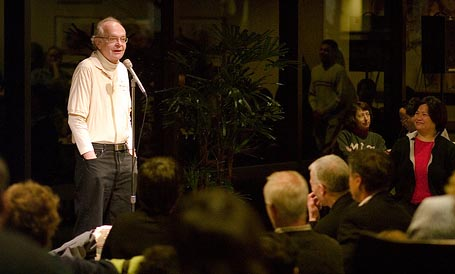
\includegraphics[width=8cm]{KnuthSpeech1990.jpg}\\
  \caption{Knuth \index{Knuth} 在 1990 年发出最终宣言}{Knuth gave the final declaration in 1990}
  \label{fig:KnuthSpeech1990}
\end{figure}


1990 年 \TeX{} \index{\TeX} 第 3.1 版发布时 (\cite{BaoTaiLei2008}), Knuth \index{Knuth} 教授发出最终宣言:
\begin{itemize}
  \item 不再对 \TeX{} \index{\TeX} 进行任何扩张;
  \item 如果出现明显问题, 修正的版本依次为 3.14 版, 3.141 版, 3.1415 版 \ldots,
        在自己离开这个世界的时候, 将最后的 \TeX{} \index{\TeX} 版本序号改为 $\pi$.
        此后, 即使再发现错误, 也都将成为 \TeX{} \index{\TeX} 的特征而保留. 如果
        有人非要修改的话, 就不要再叫 \TeX{} \index{\TeX} 了, 请另外起名.
  \item 关于 \TeX{} \index{\TeX} 的一切, 已经全部做了书面说明, 可以自由利用设计
        其他的软件.
\end{itemize}

\TeX{} \index{\TeX} 系统是由 Pascal \index{Pascal} 语言编写的, 程序的源代码也是
公开的. 它包含 300 条基本命令和 600 条扩展命令, 几乎可以排版任何形式的文献, 如一
般文章、报告、书刊和诗集等, 对数学公式的排版也被公认是最好的. \TeX{} \index{\TeX}
系统的优点之一就是它支持命令宏, 这使得使用 \TeX{} \index{\TeX} 成为一种乐趣, 用户
可以自己编写宏包来定义更多、更方便的新命令, 这也是 \TeX{} \index{\TeX} 能得以迅速
发展的原因. 而且, \TeX{} \index{\TeX} 是一个可移植的软件系统, 它可以运行于所有类
型的计算机 (如苹果机、IBM PC 机及大型工作站) 和各种操作系统 (如 DOS、Windows、
Unix 等).

\TeX{} \index{\TeX} 另一个重要特征就是它的输出是与设备无关. \TeX{} \index{\TeX}
的输出文件称为 DVI 文件, 即是``设备无关". 一旦 \TeX{} \index{\TeX} 处理了你的文
件, 所得到的 DVI 文件就可以被送到任何输出设备如打印机、屏幕等, 并且总会得到相同
的结果, 而这与这些输出设备的限制没有任何关系. 这说明 DVI 文件中所有的元素, 从页
面设置到文本中字符的位置都被固定, 不能更改.

最基本的 \TeX{} \index{\TeX} 程序只是由一些很原始的命令组成, 它们可以完成简单的
排版操作和程序设计功能. 然而, \TeX{} \index{\TeX} 也允许用这些原始命令定义一些更
复杂的高级命令. 这样就可以利用低级的块结构, 形成一个用户界面相当友好的环境.

虽然 \TeX{} \index{\TeX} 在过去的二十多年中没有大的变化, 但它开放的设计使得它能
够很容易适应新的要求.  例如, 在没有改动内核的情况下, \TeX{} \index{\TeX} 很容易
地实现了对 PostScript\index{PostScript} 字体和外部图形的支持; \TeX{} \index{\TeX}
是第一个能够自动生成 HTML 的字处理软件; 现在, \TeX{} \index{\TeX} 还可以在不
借助其它工具 (如 Adobe Distiller) 的条件下生成 PDF 格式文件.

\TeX{} \index{\TeX} 不仅是一个排版程序, 而且是一种程序语言. \LaTeX{} \index{\TeX}
就是使用这种语言写成的一个``\TeX{} \index{\TeX} 宏包", 它扩展了 \TeX{} \index{\TeX}
的功能, 使我们很方便地进行富于逻辑性的创作而不是专心于字体、缩进等这些烦人的东西.

\TeX{} \index{\TeX} 源文件是 ASCII 码文件, 可以方便地在网络上传播. 目前, 大多数
学术部分和校园网上都安装有 \TeX{} \index{\TeX} 系统. 国际上许多出版机构也采用
\TeX{} \index{\TeX} 系统来排版书刊, 不少出版社还要求作者提供稿件的 \TeX{} \index{\TeX}
源文件.
